\documentclass[Supplementary.tex]{subfiles}
\begin{document}
 \begin{figure}[ht]
     \centering
     \begin{subfigure}{0.28\textwidth}
        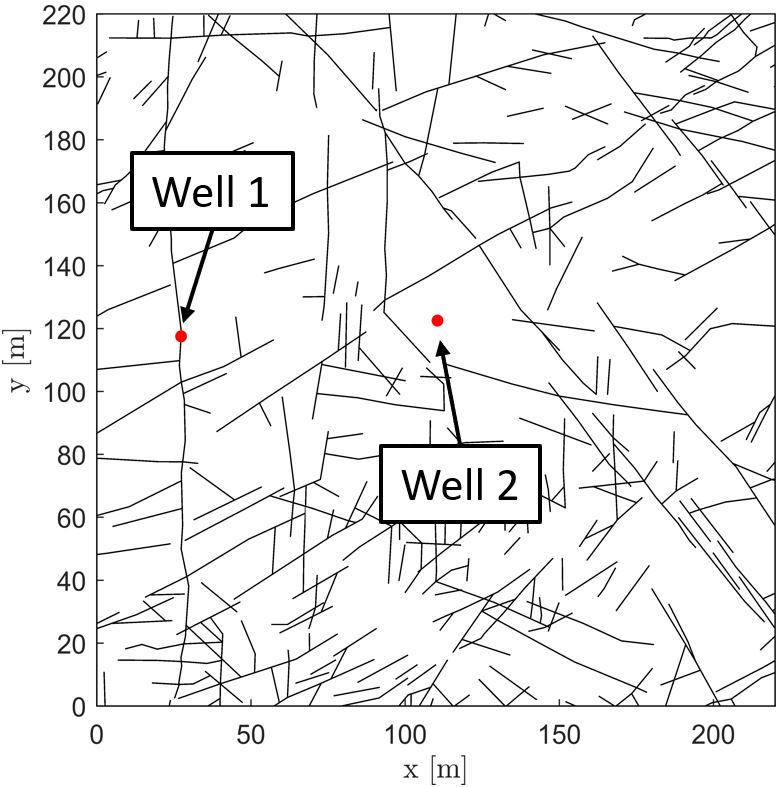
\includegraphics[width=\textwidth]{Apodi_DD/Apodi2.JPG}
        \subcaption{Apodi 2: Well Locations}
        \label{fig:Apodi2}
     \end{subfigure}
     \begin{subfigure}{0.35\textwidth}
        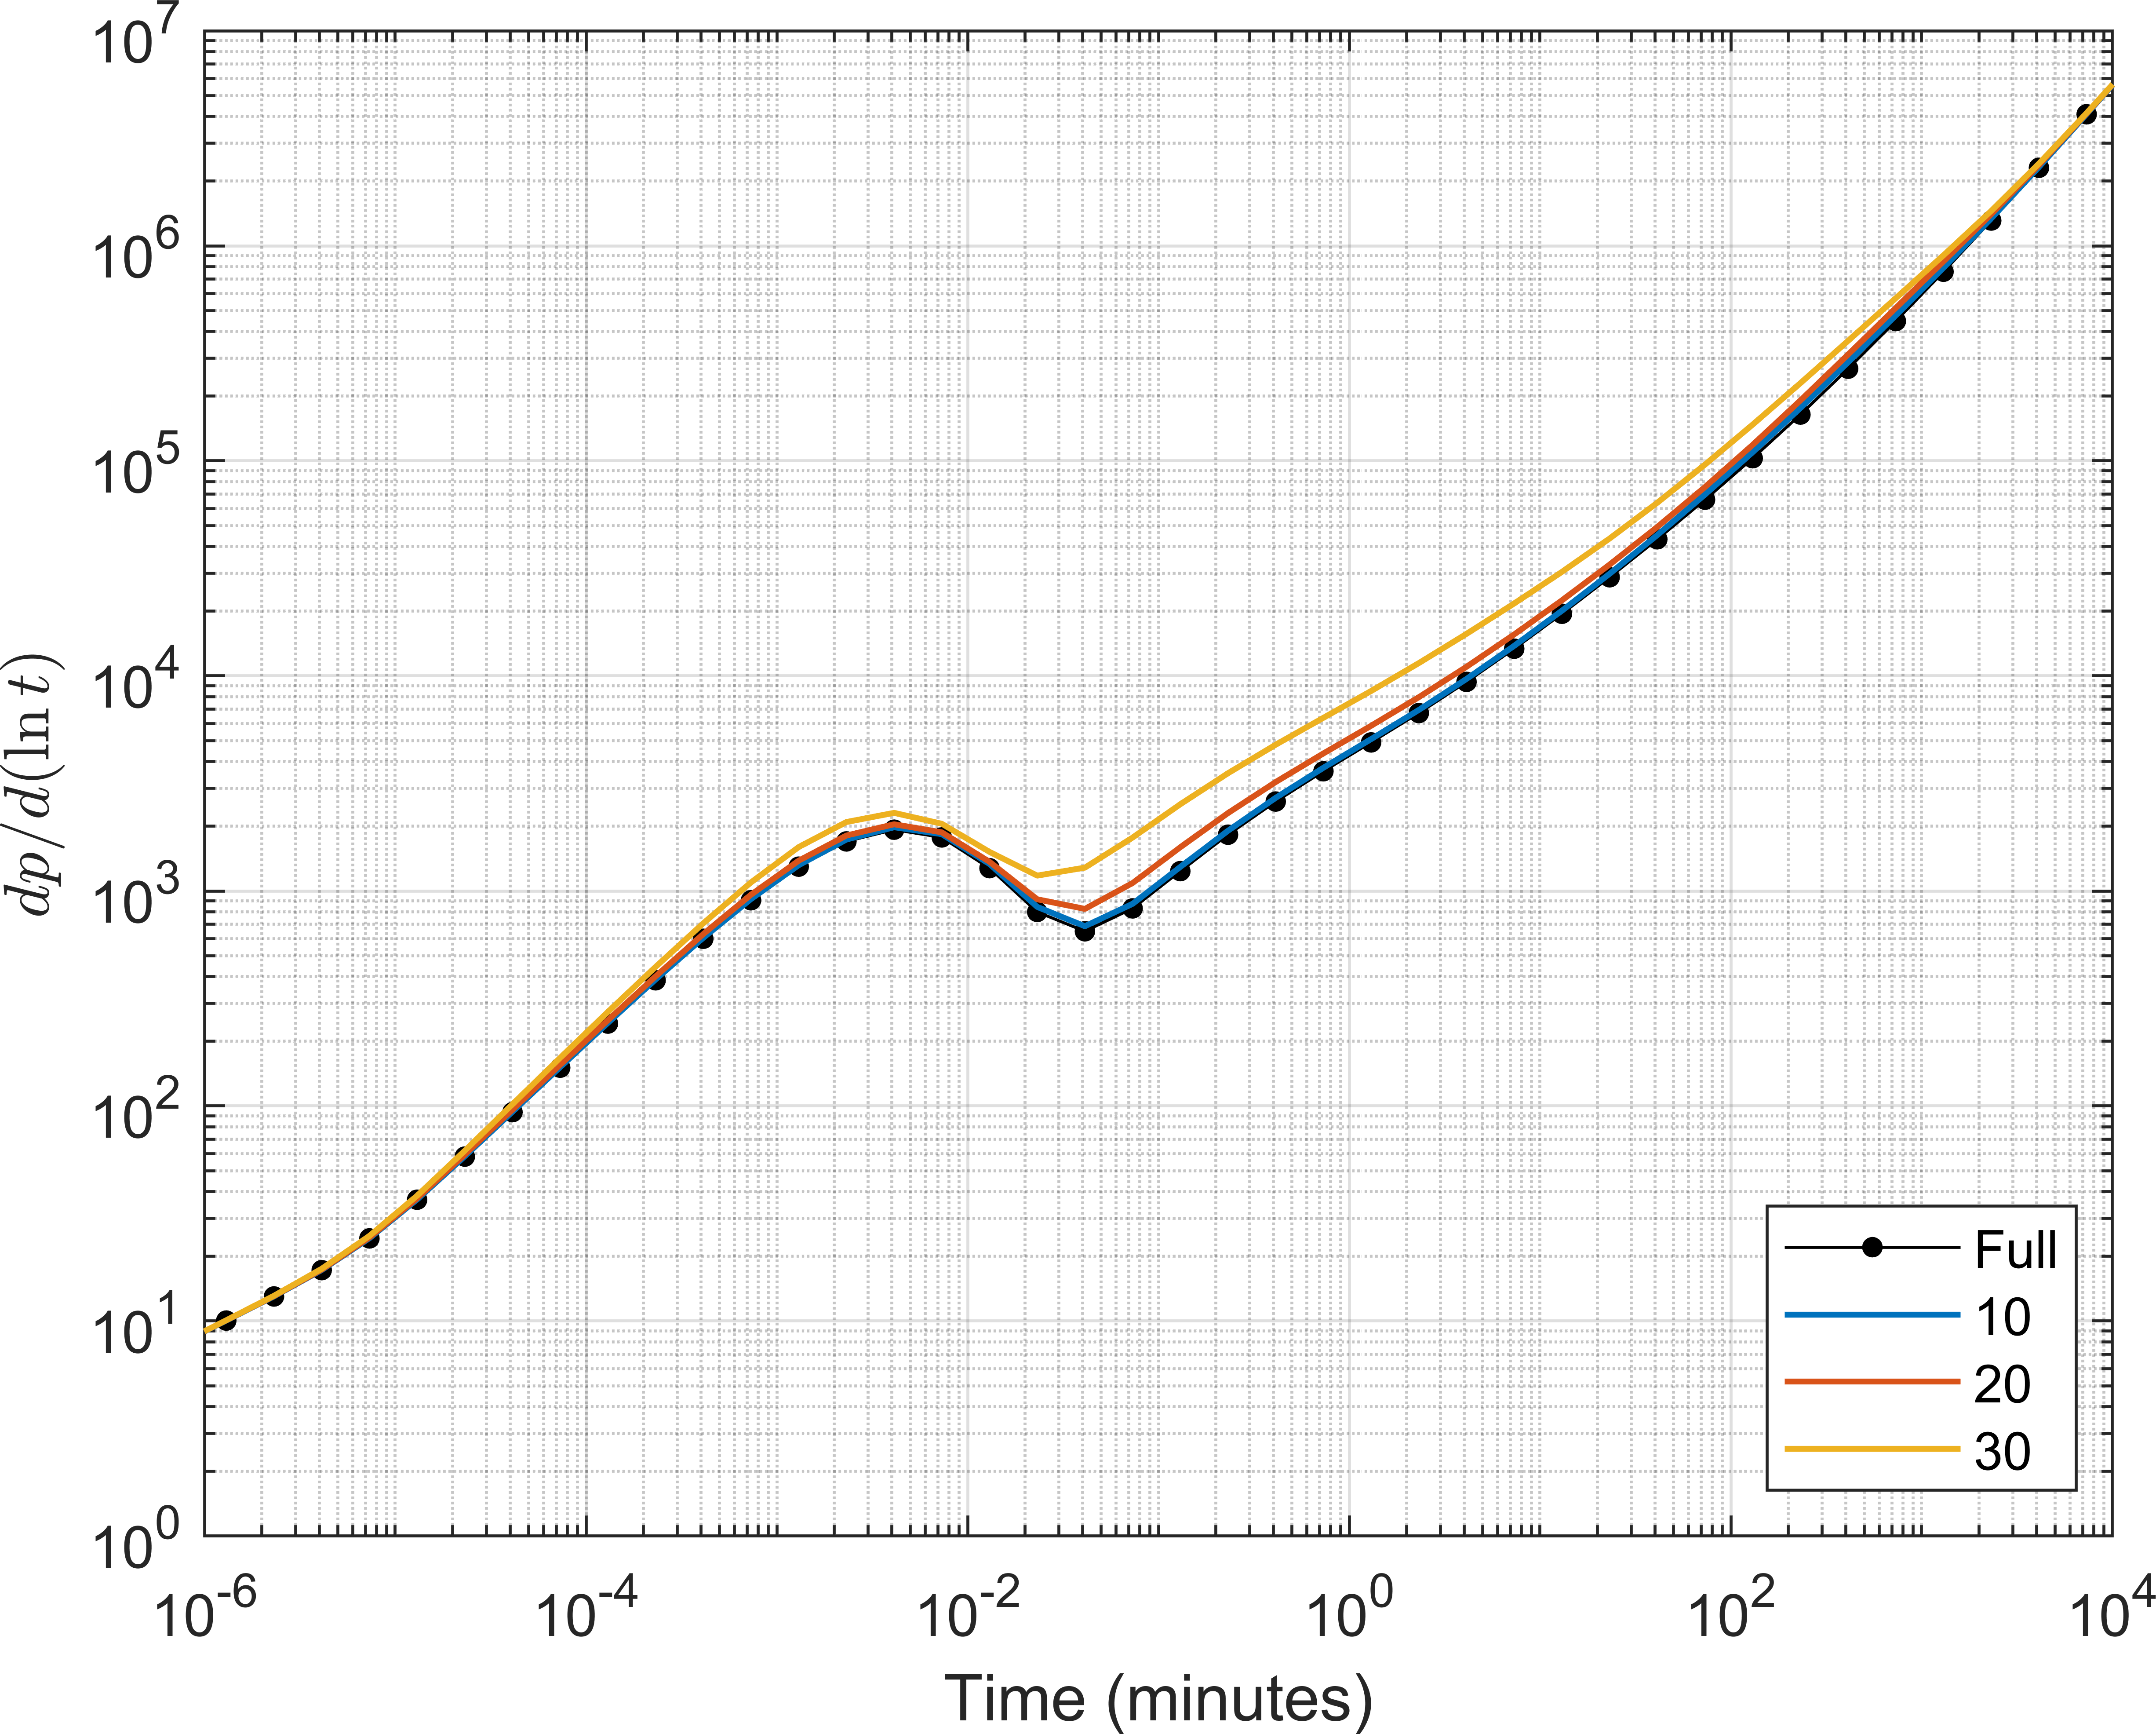
\includegraphics[width=\textwidth]{Apodi_DD/Apodi2_frac_nohead.png}
        \subcaption{Apodi 2: Well 1}
        \label{fig:Apodi2_DD_frac}
     \end{subfigure}
     \begin{subfigure}{0.35\textwidth}
        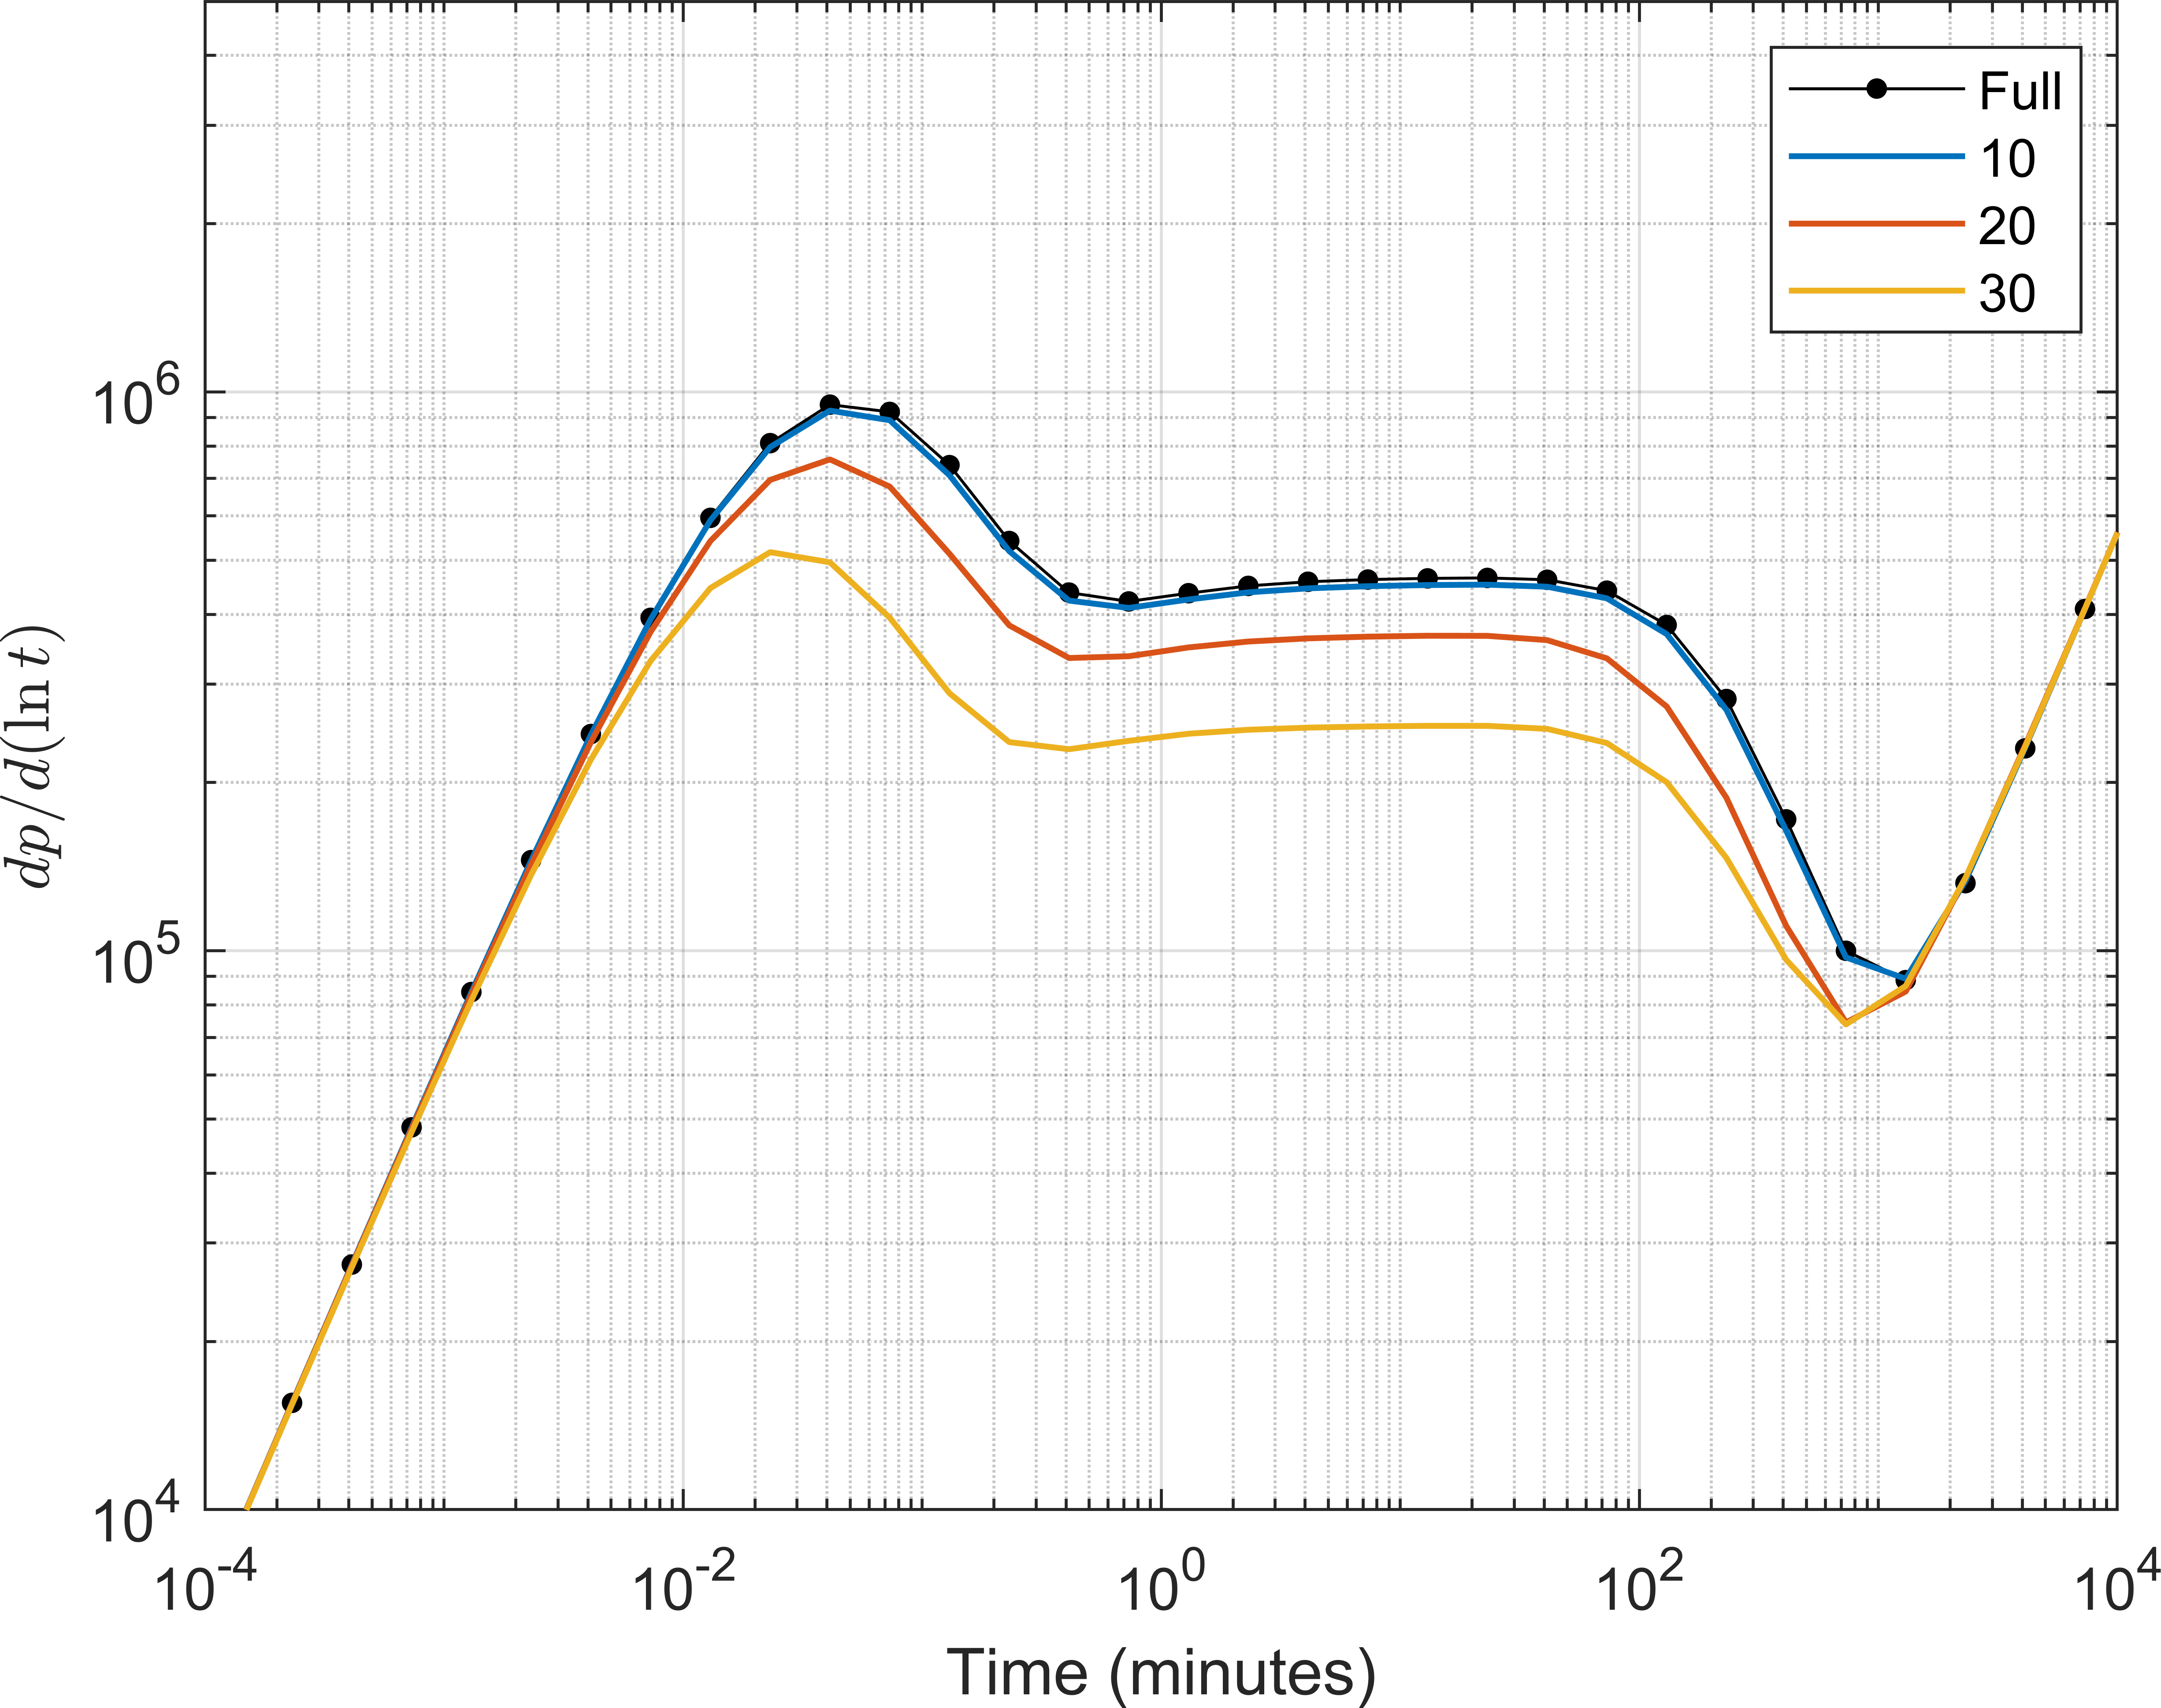
\includegraphics[width=\textwidth]{Apodi_DD/Apodi2_mat_nohead.png}
        \subcaption{Apodi 2: Well 2}
        \label{fig:Apodi2_DD_mat}
     \end{subfigure}
     \\
     \begin{subfigure}{0.285\textwidth}
        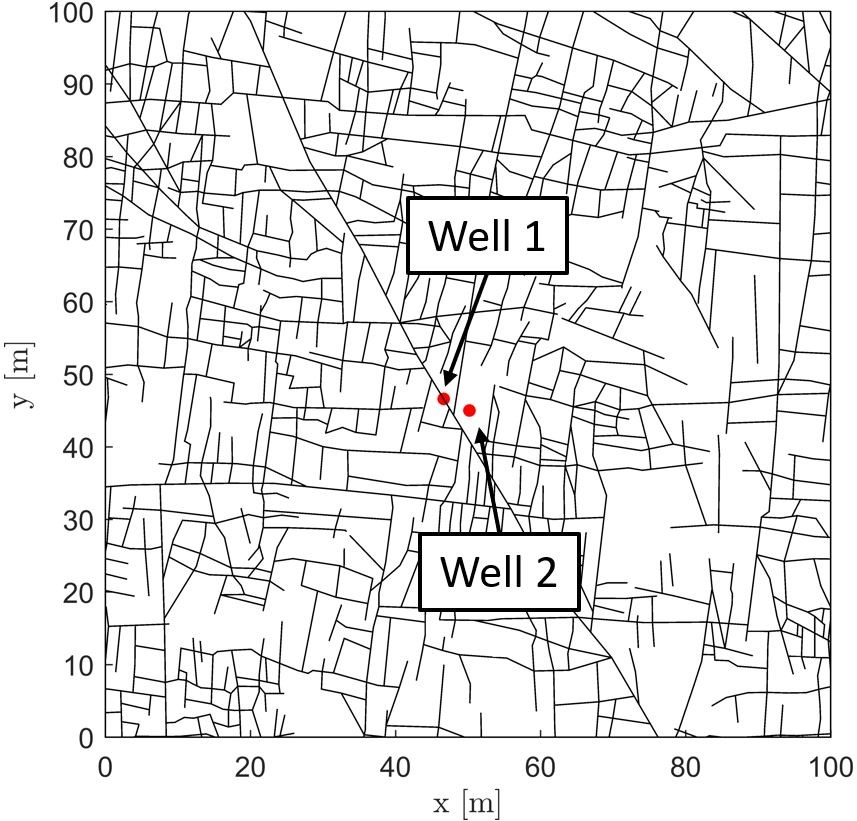
\includegraphics[width=\textwidth]{Apodi_DD/Apodi4.JPG}
        \subcaption{Apodi 4: Well Locations}
        \label{fig:Apodi4}
     \end{subfigure}
     \begin{subfigure}{0.35\textwidth}
        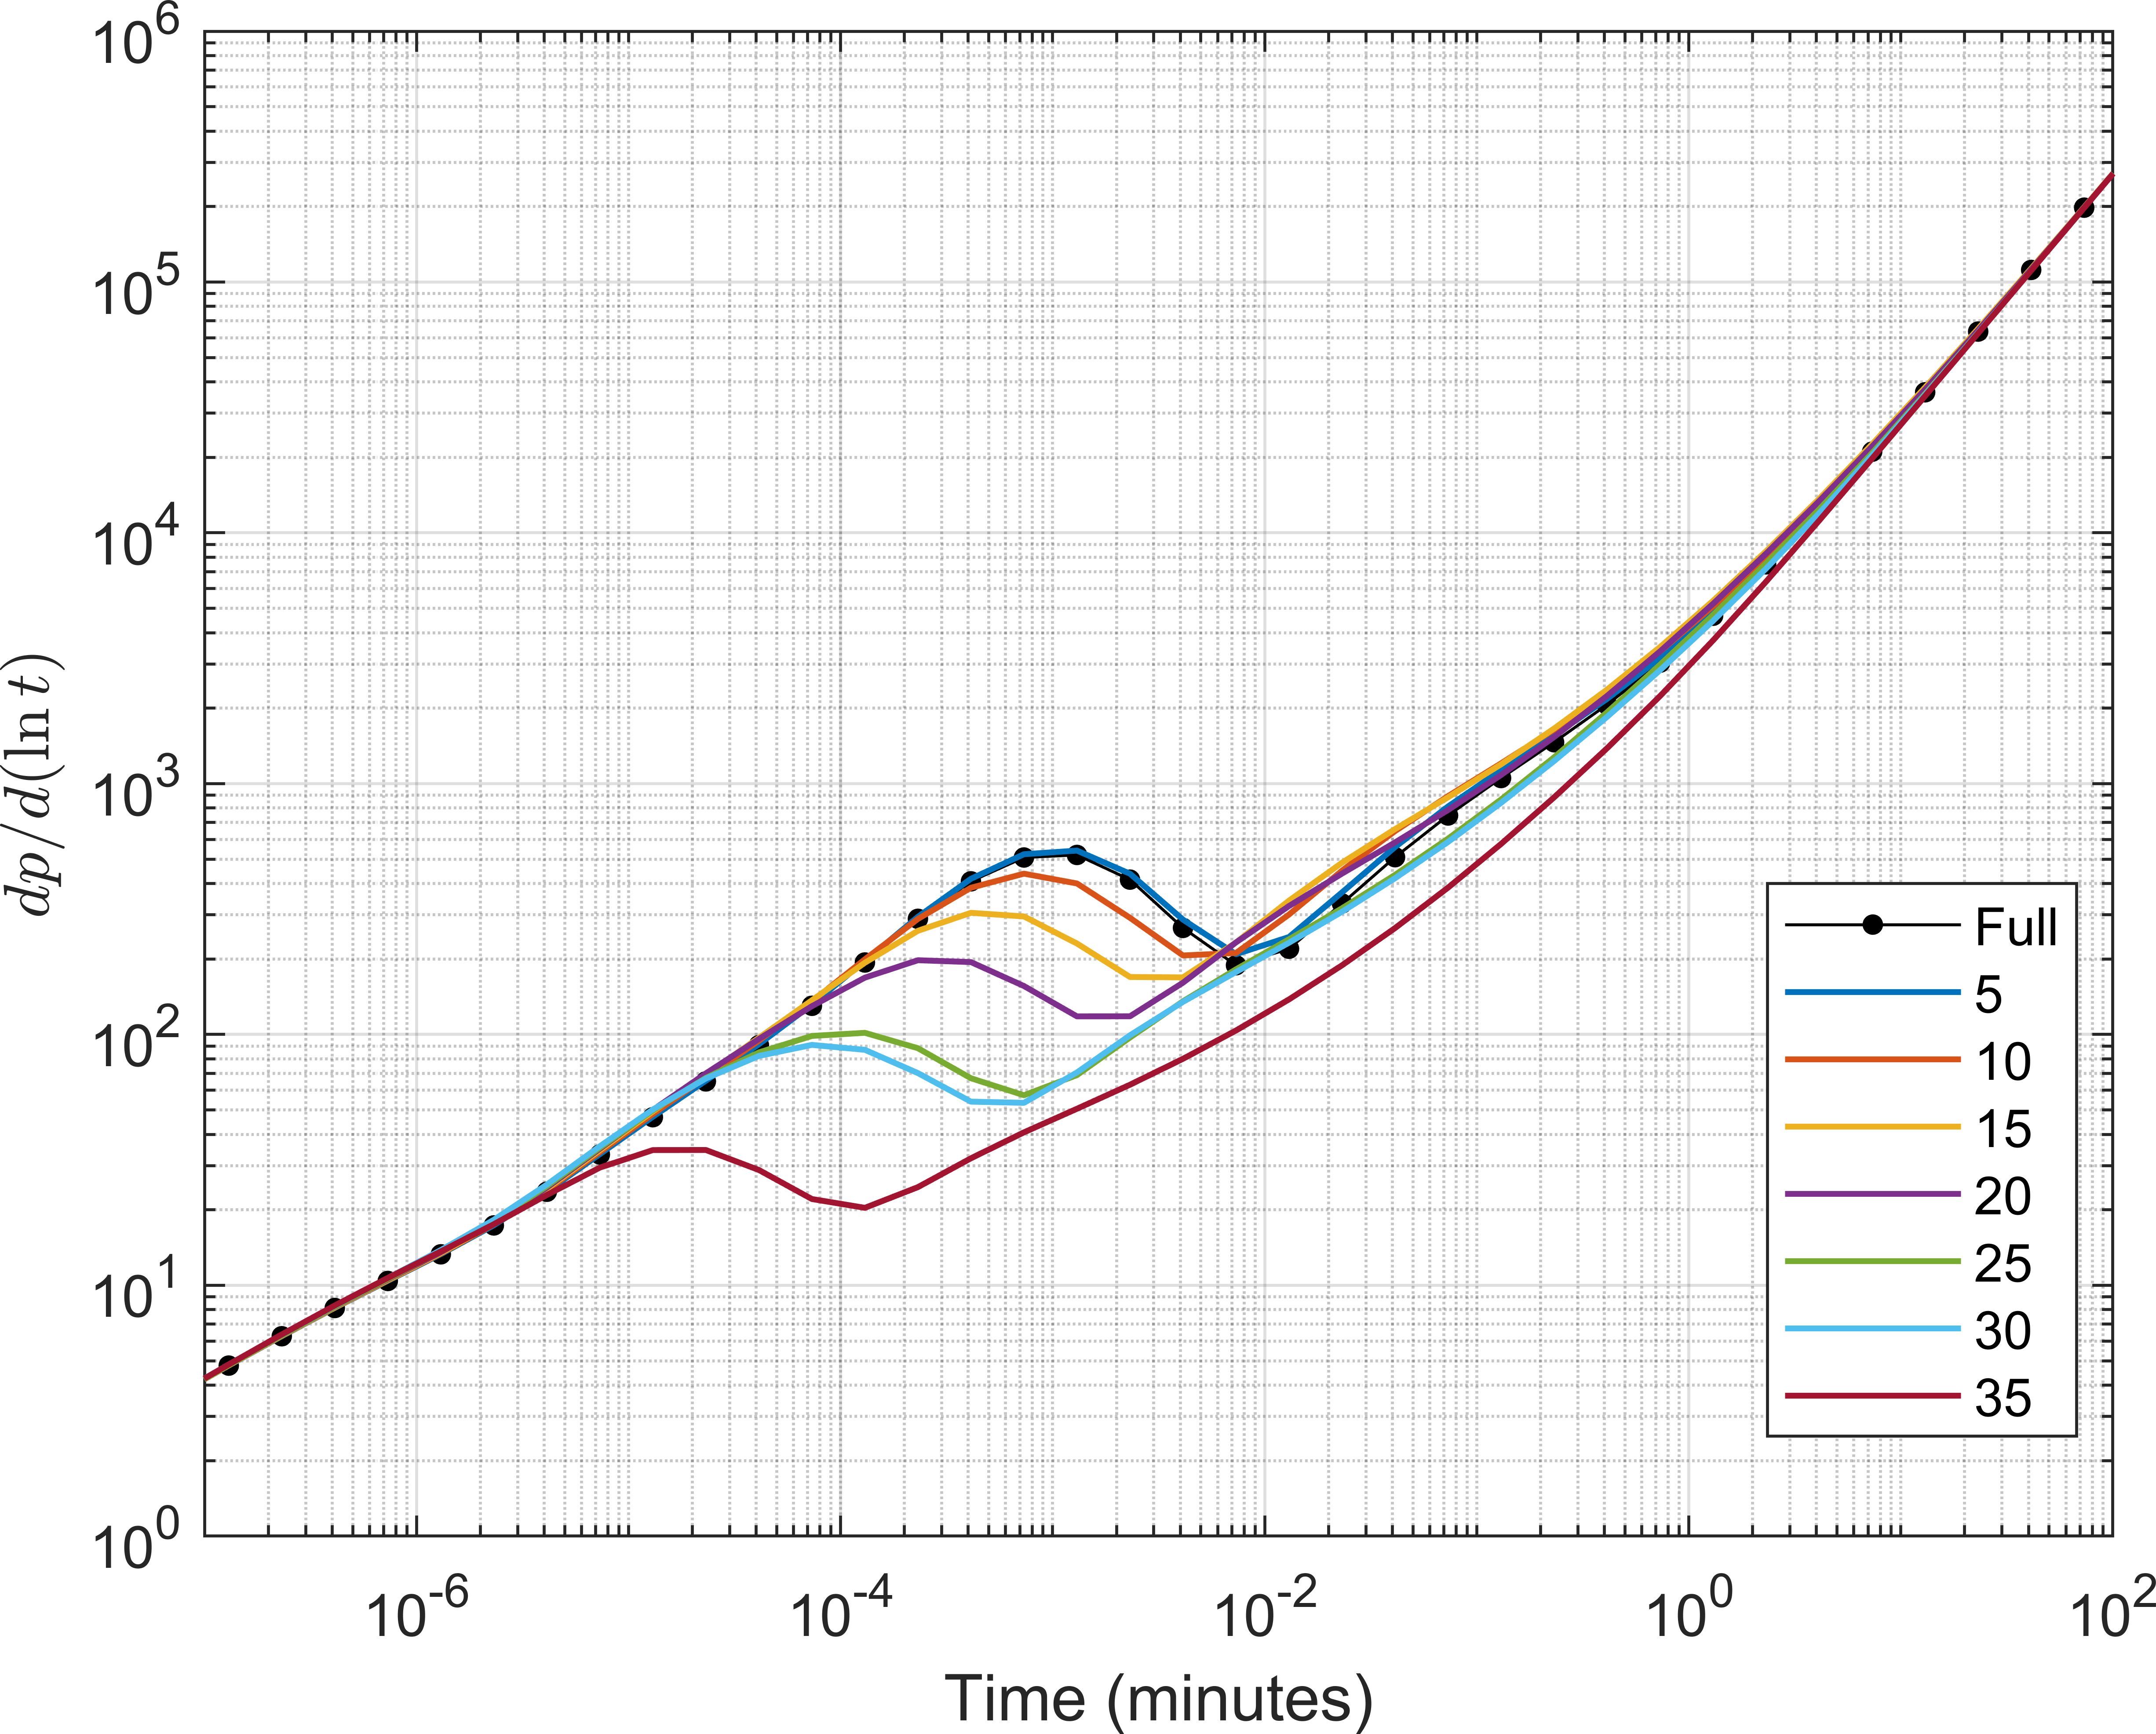
\includegraphics[width=\textwidth]{Apodi_DD/Apodi4_frac_nohead.png}
        \subcaption{Apodi 4: Well 1}
        \label{fig:Apodi4_DD_frac}
     \end{subfigure}
     \begin{subfigure}{0.35\textwidth}
        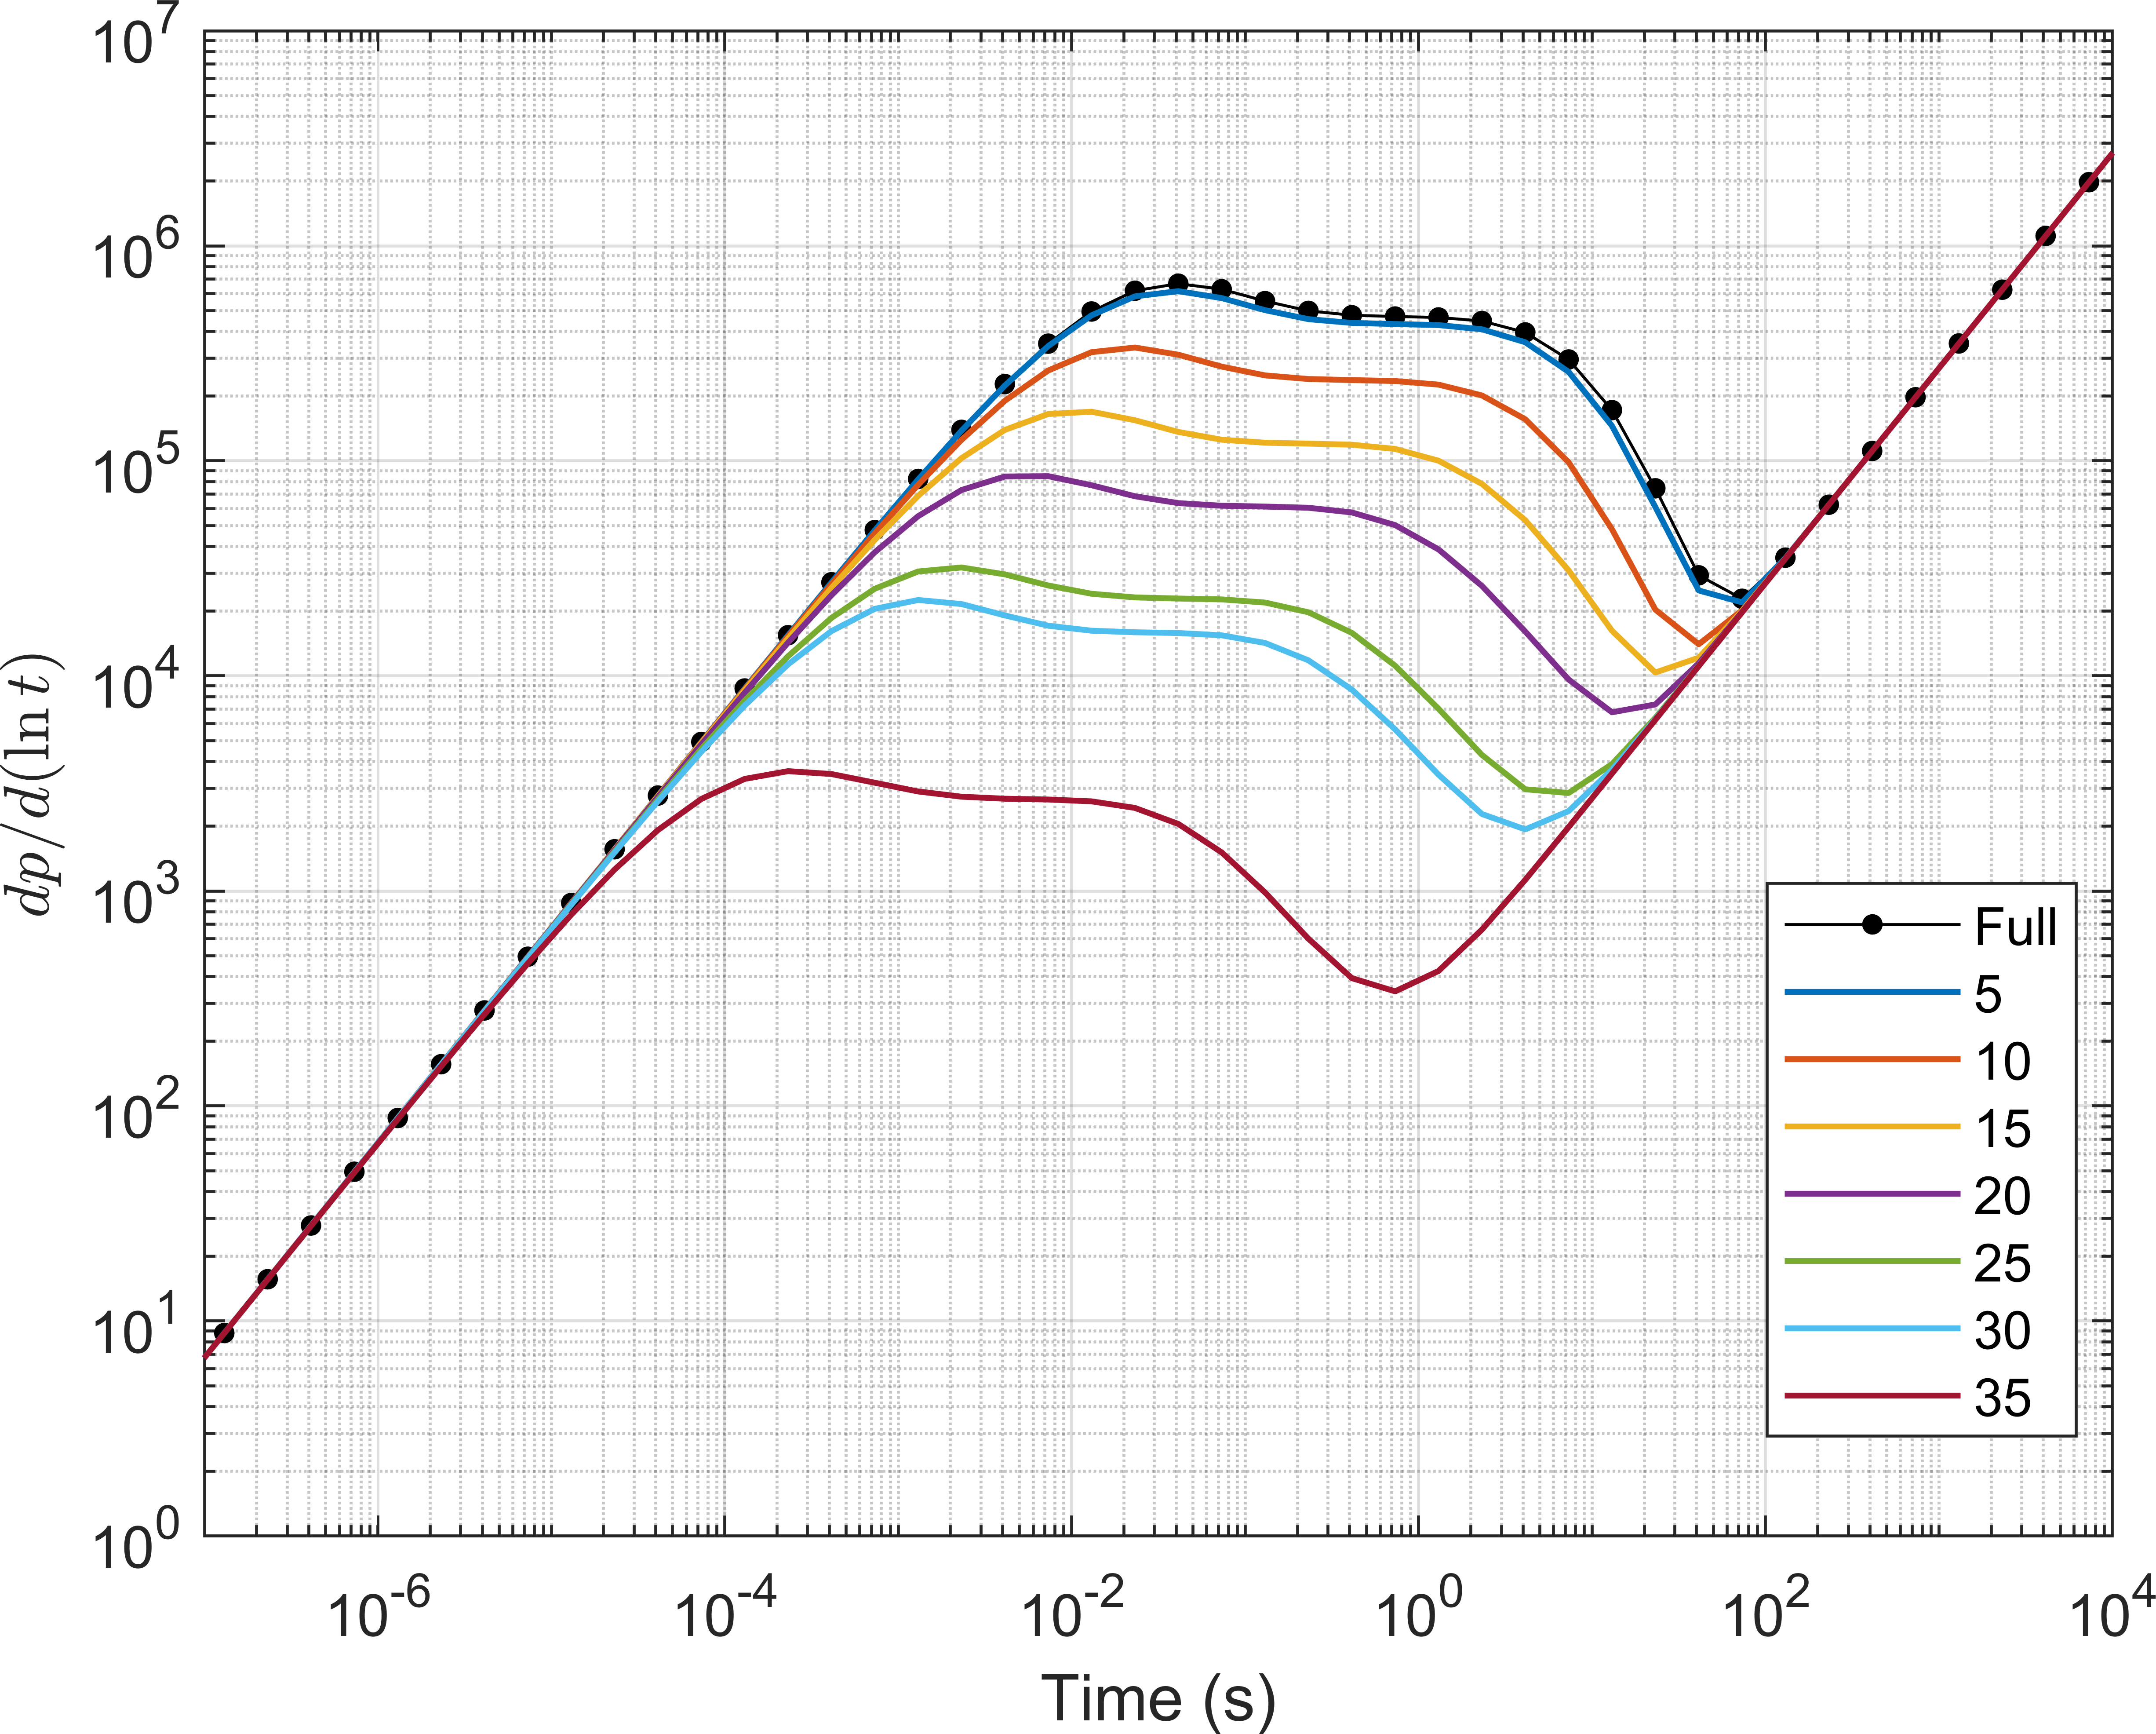
\includegraphics[width=\textwidth]{Apodi_DD/Apodi4_mat_nohead.png}
        \subcaption{Apodi 4: Well 2}
        \label{fig:Apodi4_DD_mat}
     \end{subfigure}
     \caption{Well test pressure derivative curves for outcrop based fracture networks. Each fracture network is subjected to two separate well test scenarios: Well 1 located in a fracture and Well 2 located in the matrix.}
     \label{fig:Apodi_DD}
 \end{figure}
\end{document}